\documentclass[../body.tex]{subfiles}
\begin{document}
\subsection{Нейронная сеть}
\subsubsection{Определение нейронной сети}
\textit{Нейронная сеть прямого распространения} (англ. feedforward neural network) – суперпозиция нескольких слоёв нейронов (чаще всего, сигмоидальных) (\cite{gonsales}, c. 1023). Входом каждого нейрона служит линейная комбинация выходов предыдущего слоя с добавлением \textit{свободного члена} (англ. intercept term), определяющего \textit{порог активации} нейрона. Вход первого слоя – входной вектор нейросети, выход последнего – выходной вектор (в классификационной задаче каждая компонента выходного вектора означает вероятность попадания в соответствующий класс с точки зрения нейросети). С математической точки зрения нейронная сеть – многократная суперпозиция линейных комбинаций нелинейных функций, что позволяет ей формировать границы сложной формы при решении задачи классификации.

Параметры нейросети:
\begin{enumerate}
	\item $L$ -- число слоёв
	\item $m^{(l)}$ -- число слоёв в нейроне, $l \in \{1;k\}$
	\item $g^{(l)}$ -- активационная функция, как правило, одинаковая для всех нейронов слоя $l$
	\item $W^{(l)}$ -- матрица весов при переходе от слоя $l$ к $l+1$
\end{enumerate}

Веса $W^{(l)}$ выбираются в процессе обучения. Остальные параметры остаются постоянными. На рис. \ref{nnetNeuron} показано схематическое изображение нейрона. 

\begin{figure}[H]
	\center{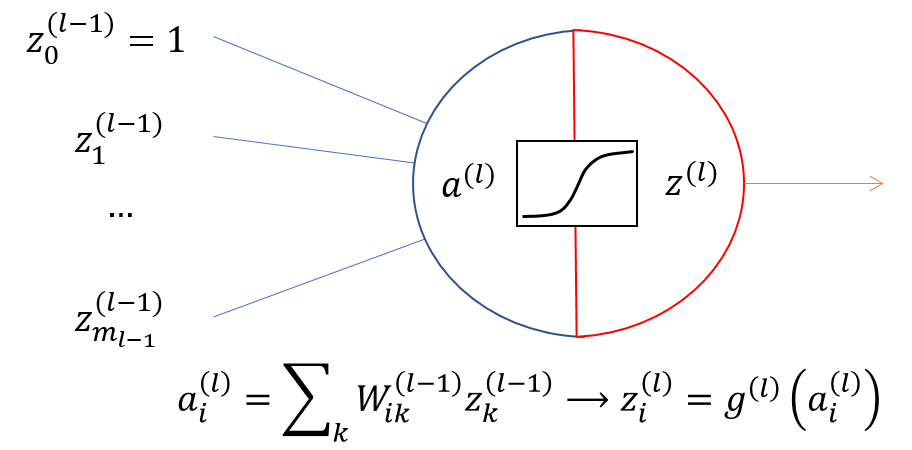
\includegraphics[width=.5\textwidth]{img/neuron.png}}
	\caption{Графическая интерпретация нейрона}
	\label{nnetNeuron}
\end{figure}

Обучение заключается в минимизации функции ошибки $J((x_n,y_n))$, где $(x_n,y_n)$ – тренировочная пара данных: $x_n$ – входной вектор, $y_n$ – желаемый выходной вектор. В задаче классификации $y_n$ – бинарный вектор, в котором все компоненты равны нулю, кроме одной, которая задаёт класс входного вектора. Функция ошибки задаётся формулой
$$J((x_n,y_n))=\sum_{n=1}^{N}\sum_{k=1}^{K}{J_{nk}(W_k^{(L)}| x_{nk},y_{nk})}$$
где $J_{nk}(W_k^{(L)}| x_n,y_{nk})$ – вклад k-ой компоненты выходного вектора и только одного тренировочного экземпляра. Если функции активации выходного слоя $g_k^{(l)}(x)=\sigma(x)$, то в простейшем случае принимают $J_{nk}=-y_{nk}ln\cdot({\widetilde{y}}_{nk})$, где ${\widetilde{y}}_{nk}= h{(x_n|\{W^{(l)}))}_k$ – к-я компонента выходного вектора нейросети при данных значениях весов. Минимум $J_{nk}$ соответствует максимальной близости $y_{nk}$ и ${\widetilde{y}}_{nk}$. Оказывается, что функция ошибки, заданная таким образом, в общем случае имеет большое количество локальных минимумов, но при достаточном количестве тренировочных данных и применении некоторых техник (многократная случайная инициализация параметров, модификации градиентного спуска) удаётся итерационными методами найти глобальный или близкий по значению $J$ к глобальному минимум.

\subsubsection{Алгоритм обратного распространения ошибки}
Выведем алгоритм вычисления градиентов нейросети, называемый в литературе \textit{алгоритмом обратного распространения ошибки} \cite{gonsales} \cite{murphy}. В рамках данной работы ограничимся рассмотрением нейросети, состоящей только из двух слоёв нейронов (рис. \ref{nnetLayers}), причём в каждом слое функцией активации будет сигмоида.

\begin{figure}[H]
	\center{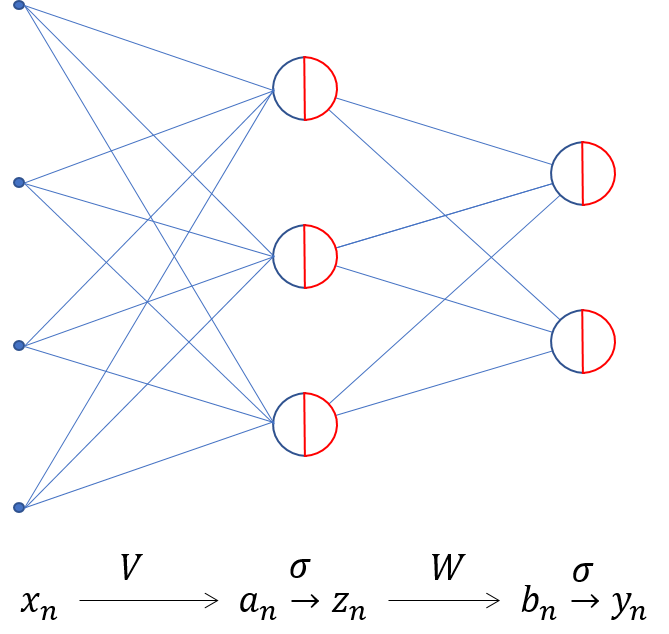
\includegraphics[width=.7\textwidth]{img/nnet.png}}
	\caption{Модель нейронной сети с двумя слоями нейронов}
	\label{nnetLayers}
\end{figure}

Здесь будем использовать следующие обозначения:\\
\begin{itemize}
	\item $x_n$ -- n-ый экземпляр входного вектора в тренировочной выборке
	\item $V, W$ -- матрицы весов на входе I и II слоёв соответственно
	\item $\theta$ -- вектор, составленный из всех значений $V$ и $W$ (минимизируется $J(\theta)$)
	\item $a_n=Vx_n$ -- вектор аргументов сигмоиды
	\item $z_n=\sigma(a_n)$ -- активации в I слое: значение сигмоиды, применяемой покомпонентно
	\item $b_n=Wz_n$ -- входы II слоя
	\item ${\widetilde{y}}_n=\sigma(b_n)$ -- выходной вектор нейросети при входном значении $x_n$.
\end{itemize}

Функция стоимости в данном случае
$$J=-\frac{1}{m}\sum_{n}\sum_{k} y_{nk}ln({\widetilde{y}}_{nk})$$
Требуется найти $\mathrm{\nabla}_\mathrm{\theta}J$. Поскольку $J=-\sum_{n} J_n$, найдём $\mathrm{\nabla}_\mathrm{\theta}J_n$, где $J_n$ – вклад одного экземпляра тренировочных данных:
$$J_n=-\sum_{k} y_{nk}ln({\widetilde{y}}_{nk})=-\sum_{k} y_{nk}ln(\sigma(b_{nk}))=-\sum_{k} y_{nk}ln(\sigma(W_kz_n))$$
Градиенты коэффициентов, задающих переход от первого (скрытого) слоя ко второму:
$$\mathrm{\nabla}_{\mathrm{Wk}}J_n=\frac{\partial J_n}{\partial b_{nk}}\mathrm{\nabla}_{\mathrm{Wk}}b_{nk}=\frac{\partial J_n}{\partial b_{nk}}z_n$$
Введём $\delta_{nk}^W\overset{def}{=}\frac{\partial J_n}{\partial b_{nk}}$. Несложно показать, что $$\delta_{nk}^W=-(y_{nk}ln(\sigma(b_{nk})))_{b_{nk}}^\prime=y_{nk}-{\widetilde{y}}_{nk}$$
Градиенты коэффициентов матрицы $V$
$$\mathrm{\nabla}_{Vj}J_n=\frac{\partial J_n}{\partial a_{nj}}\nabla_{Vj}a_{nj}$$
Введём $\delta_{nj}^V\overset{def}{=}\frac{\partial J_n}{\partial a_{nj}}$. Тогда, поскольку $a_{nj}=V_jx_n$,
$$\nabla_{Vj}J_n=\delta_{nj}^Vx_n
\delta_{nj}^V=\frac{\partial J_n}{\partial a_{nj}}=\sum_{k}{\frac{\partial J_n}{\partial b_{nk}}\frac{\partial b_{nk}}{\partial a_{nj}}}=\sum_{k}{\delta_{nk}^W\frac{\partial b_{nk}}{\partial a_{nj}}}$$
$$b_{nk}=\sum_{j} W_{kj}\sigma(a_{nj})arrow\frac{\partial b_{nk}}{\partial a_{nj}}=W_{kj}\sigma^\prime(a_{nj})=W_{kj}\sigma(a_{nj})(1-\sigma(a_{nj}))$$
$$\delta_{nj}^V=\sum_{k}\delta_{nk}^WW_{kj}\sigma(a_{nj})(1-\sigma(a_{nj}))$$
Получив выражения для $\delta_{nk}^W и \delta_{nj}^V$, вычисляем вектор градиента:
$$\mathrm{\nabla}_\mathrm{\theta}J=\frac{1}{m}((\nabla_{Wk}J_n) (\nabla_{Vj}J_n))=\frac{1}{m}((\delta_{nk}^Wz_n) (\delta_{nj}^Vx_n) )$$
\textbf{Замечание}. Если в нейронной сети более двух слоёв и $x_n$ – не входные данные, а выходы предыдущего слоя, аналогично можно выразить градиенты коэффициентов предыдущих матриц, узнав ошибки очередного предыдущего слоя $\delta_{nm_l}^{W^{(l)}}$ через ошибки следующего слоя $\delta_{nm_{l+1}}^{W^{(l+1)}}$.


\subsubsection{Пример обучения нейронной сети}
Приведём пример построения классификационной нейросети. Для наглядности выбран массив двумерных данных – 100 точек на плоскости с распределением в два класса (источник: \url{https://coursera.org/learn/machine-learning/}), поэтому входной вектор $x\in R^2$.  Построена двухслойная нейросеть: в первом слое (единственном скрытом) $m_1$ сигмоидальных нейронов, во втором (выходном) один сигмоидальный нейрон. Веса изначально инициализированы случайными значениями в диапазоне $(-\varepsilon;+\varepsilon)$, где $\varepsilon=0.12$ (значение выведено эмпирически на основании того, что веса вначале должны быть близки к нулю, но ненулевые, поскольку при нулевых весах градиент $\nabla_\theta J=\vec{0}$). На рис. \ref{nnetBoundary}  показано выходное значение нейросети при $m_1=5$ после 50 итераций градиентного спуска ($J\ \approx0.359$).
\begin{figure}[H]
	\center{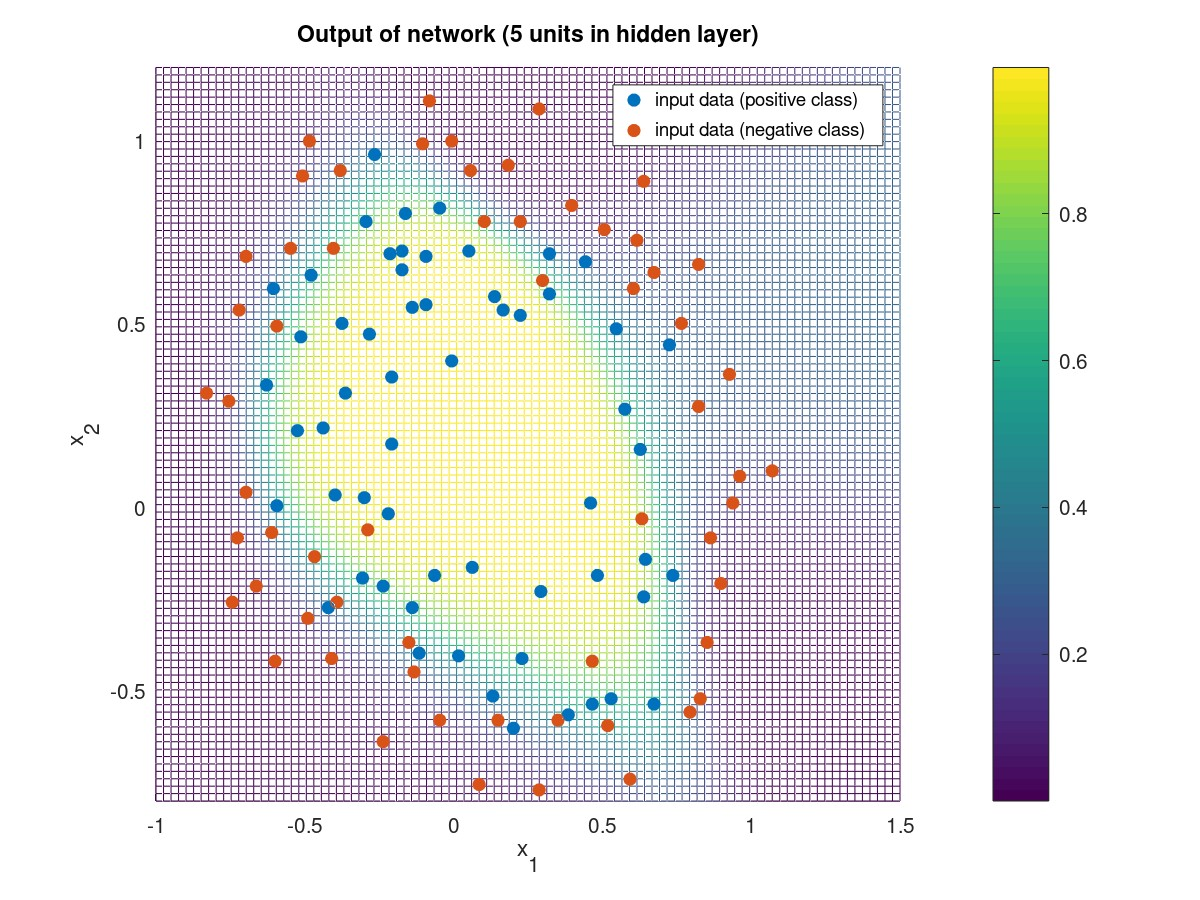
\includegraphics[width=.9\textwidth]{img/nnet_boundary.jpg}}
	\caption{Значение гипотезы, формируемой нейросетью, и тренировочные данные}
	\label{nnetBoundary}
\end{figure}
\end{document}